\hypertarget{funnel-metadynamics-tutorial}{%
\label{funnel-metadynamics-tutorial}}
\hypertarget{Introduction}{%
\subsubsection{Introduction}\label{Introduction}}

Funnel metadynamics (fun-metaD) is a molecular dynamics-based method
that calculates the absolute binding free energy (ABFE) between a small
organic ligand and a protein. It uses an enhanced sampling method called
metadynamics, which speeds up the molecular processes of interest by
periodically adding small amounts of bias. To best separate the bound
and unbound phases, as well as increase the rate of convergence, the
exploration of the ligand in 3D space is limited by funnel-shaped
restraints.

This tutorial paper describes how to set up and analyze fun-metaD
simulations. fun-metaD was originally described by Limogelli \emph{et al}~\cite{Limongelli2013}.
This tutorial follows the implementation described by Rhys \emph{et al}~\cite{Evans2020}, and Saleh \emph{et al}~\cite{Saleh2017}. The main difference between the original and later 
implementations is the functional form of the funnel restraints: the
original fun-metaD relied on a cone and a cylinder joined to make a
funnel using a step function, while the new implementation uses a single
sigmoid function. The Limogelli implementation also requires the protein
to be realigned with a reference structure to keep the funnel strictly
in place over the binding site, which negatively affects performance. The
implementation described here allows the funnel to move with the
protein.

Up to now, one of the biggest drawbacks to using fun-metaD for
large-scale absolute binding free energy (ABFE) calculations were the
difficulty in setting up the simulations. It is hard to know where the funnel should be defined, how big it needs to be, and what each of the
sigmoid function parameters should be set to, along with the chore of
writing PLUMED files, where each protein and ligand system will have
slightly different atom IDs. BioSimSpace has made the setup process easier, 
automatically defining the funnel using abstract features of the 
protein cavity, assigning the relevant atom IDs, suggesting reasonable 
default funnel parameters and allowing the visualisation of the funnel restraints inside
a Jupyter Notebook. All this leads to a quicker setup and much 
faster automation of large ABFE screening campaigns.

By the end of this tutorial, you should know 1. The basics of what
fun-metaD does. 2. How to set up fun-metaD simulations and how to
visualise the funnel restraints. 3. How to analyse the results of a
fun-metaD simulation.

\hypertarget{the-theory}{%
\subsubsection{The Theory}\label{the-theory}}

Metadynamics is an enhanced sampling method that biases a simulation
along a chosen set of reaction coordinates, or as MetaD practitioners
call them, collective variables (CVs). This bias is deposited at defined
time intervals and takes the shape of a Gaussian potential.
Investigation of drug binding should involve at least one CV, the distance
from the drug molecule to the protein, where the distance between them
can be biased, causing the drug to unbind. However, that single distance
is degenerate, meaning many different configurations of the drug in 3D
space will not be described by that single distance. It also involves
the exploration of a very large volume, hindering convergence.

Fun-metaD gets around both of these problems, restricting the
exploration by using funnel-shaped restraints and reducing degeneracy by
using two CVs - `projection' and `extent'. See Figure \ref{fig:funnel}.

\begin{figure}[htp]
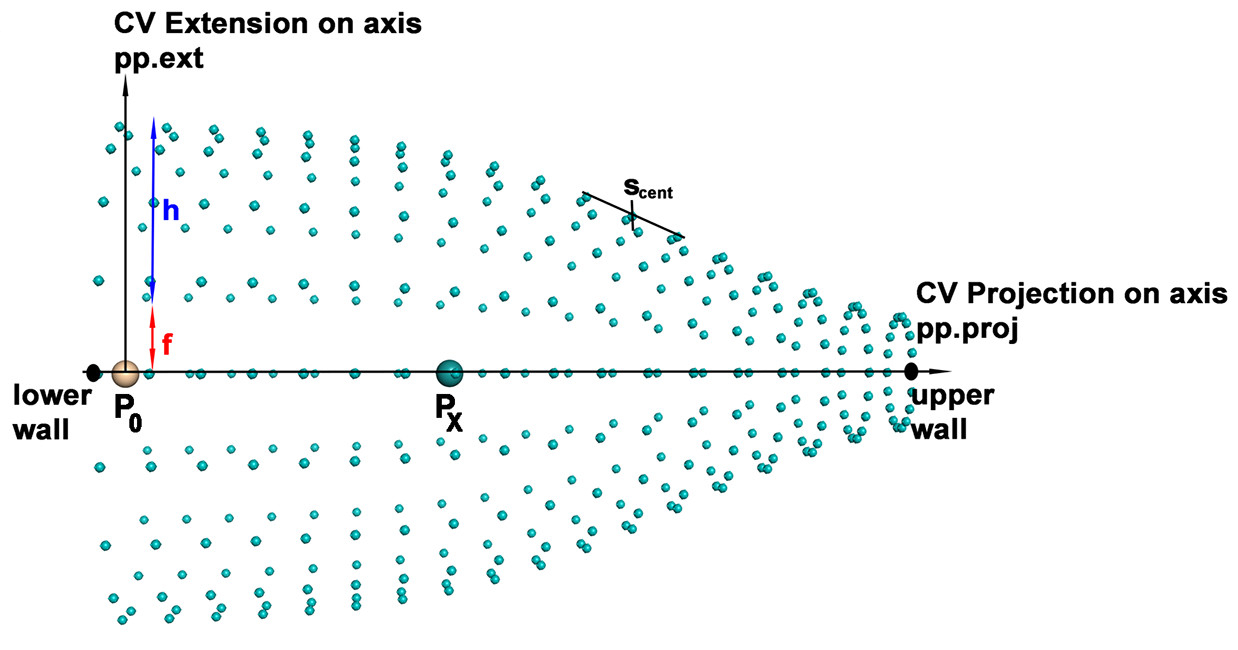
\includegraphics[width=\linewidth]{LIVECOMS/02_funnel_metad/funmetadfig1.jpeg}
\caption{Visualised funnel restraints.}
\label{fig:funnel}
\end{figure}

The restraints that limit the extent CV follow a sigmoid function:

\begin{equation}
S = h\left(\frac{1}{1+b^{b(i-x)}}\right) + f,
\end{equation}

where $S$ is the maximal distance from the axis, at pp.proj = i, h is the
`wall\_width', $f$ is the `wall\_buffer', $b$ is the `beta\_cent' (the
steepness at the inflection point), $x$ is the `s\_cent' (the inflection
point as a value of pp.proj). The exploration along pp.proj is
limited by the `lower\_wall' and `upper\_wall' parameters. The funnel's
radius at the narrow end is equal to `wall\_buffer'. `P0' and `Px' are
the points that define the funnel's vector. From now on these are referred to
as p0 and p1, respectively.

Clearly, there is still some degeneracy in the CVs - the plane
perpendicular to the projection axis is a one-dimensional representation of a two-dimensional space. However, this is a good compromise between having sufficient accuracy for describing the binding of a
ligand and the tolerable simulation slowdown of using only two CVs.

In order to have a good separation between the bound and unbound phases for the ABFE estimations, the funnel needs to point `out', with the narrow end in the solvent,
and away from any protein residues. The BSS automated funnel assignment code does this generally well. In general, the vectors picked for defining the p0 and p1 points offer an unobstructed exit path for the ligand. It is nonetheless still a good idea to visually check the proposed funnel, especially for new protein systems. This can be done through use of the funnel visualisation functionality within BSS (see below).

The size of the funnel radius has to be determined on a case-by-case basis.
In general, the funnel will look smaller than it seems necessary. The metadynamics code tracks the exploration of the center of mass of the ligand, so the volume that the small molecule will explore is much larger than implied by the visualization of the funnel. There is usually only one binding site and the funnel should enclose only it, excluding other protein
features, by setting a small `wall\_width'. This helps accelerate convergence by preventing the ligand from exploring irrelevant
regions in the free energy surface (FES). Other funnel parameters do not influence convergence as significantly and the default settings will suffice in most situations.

\hypertarget{setupfunmetad}{%
\subsubsection{Setting up funnel metadynamics simulations}\label{setupfunmetad}}

The first tutorial notebook \href{https://github.com/OpenBioSim/BioSimSpaceTutorials/blob/main/02_funnel_metad/01_bss-fun-metad-setup.ipynb}{01-bss-fun-metad-setup} describes how to set up the BioSimSpace system, parameterizing the protein and the ligand, as well as defining the simulation box, adding water and ions. A funnel is then defined and visualized using NGLview. Finally, directories for the fun-metaD simulation are setup and a short 10 ps simulation is run for illustrative purposes.


\begin{figure}[htp]
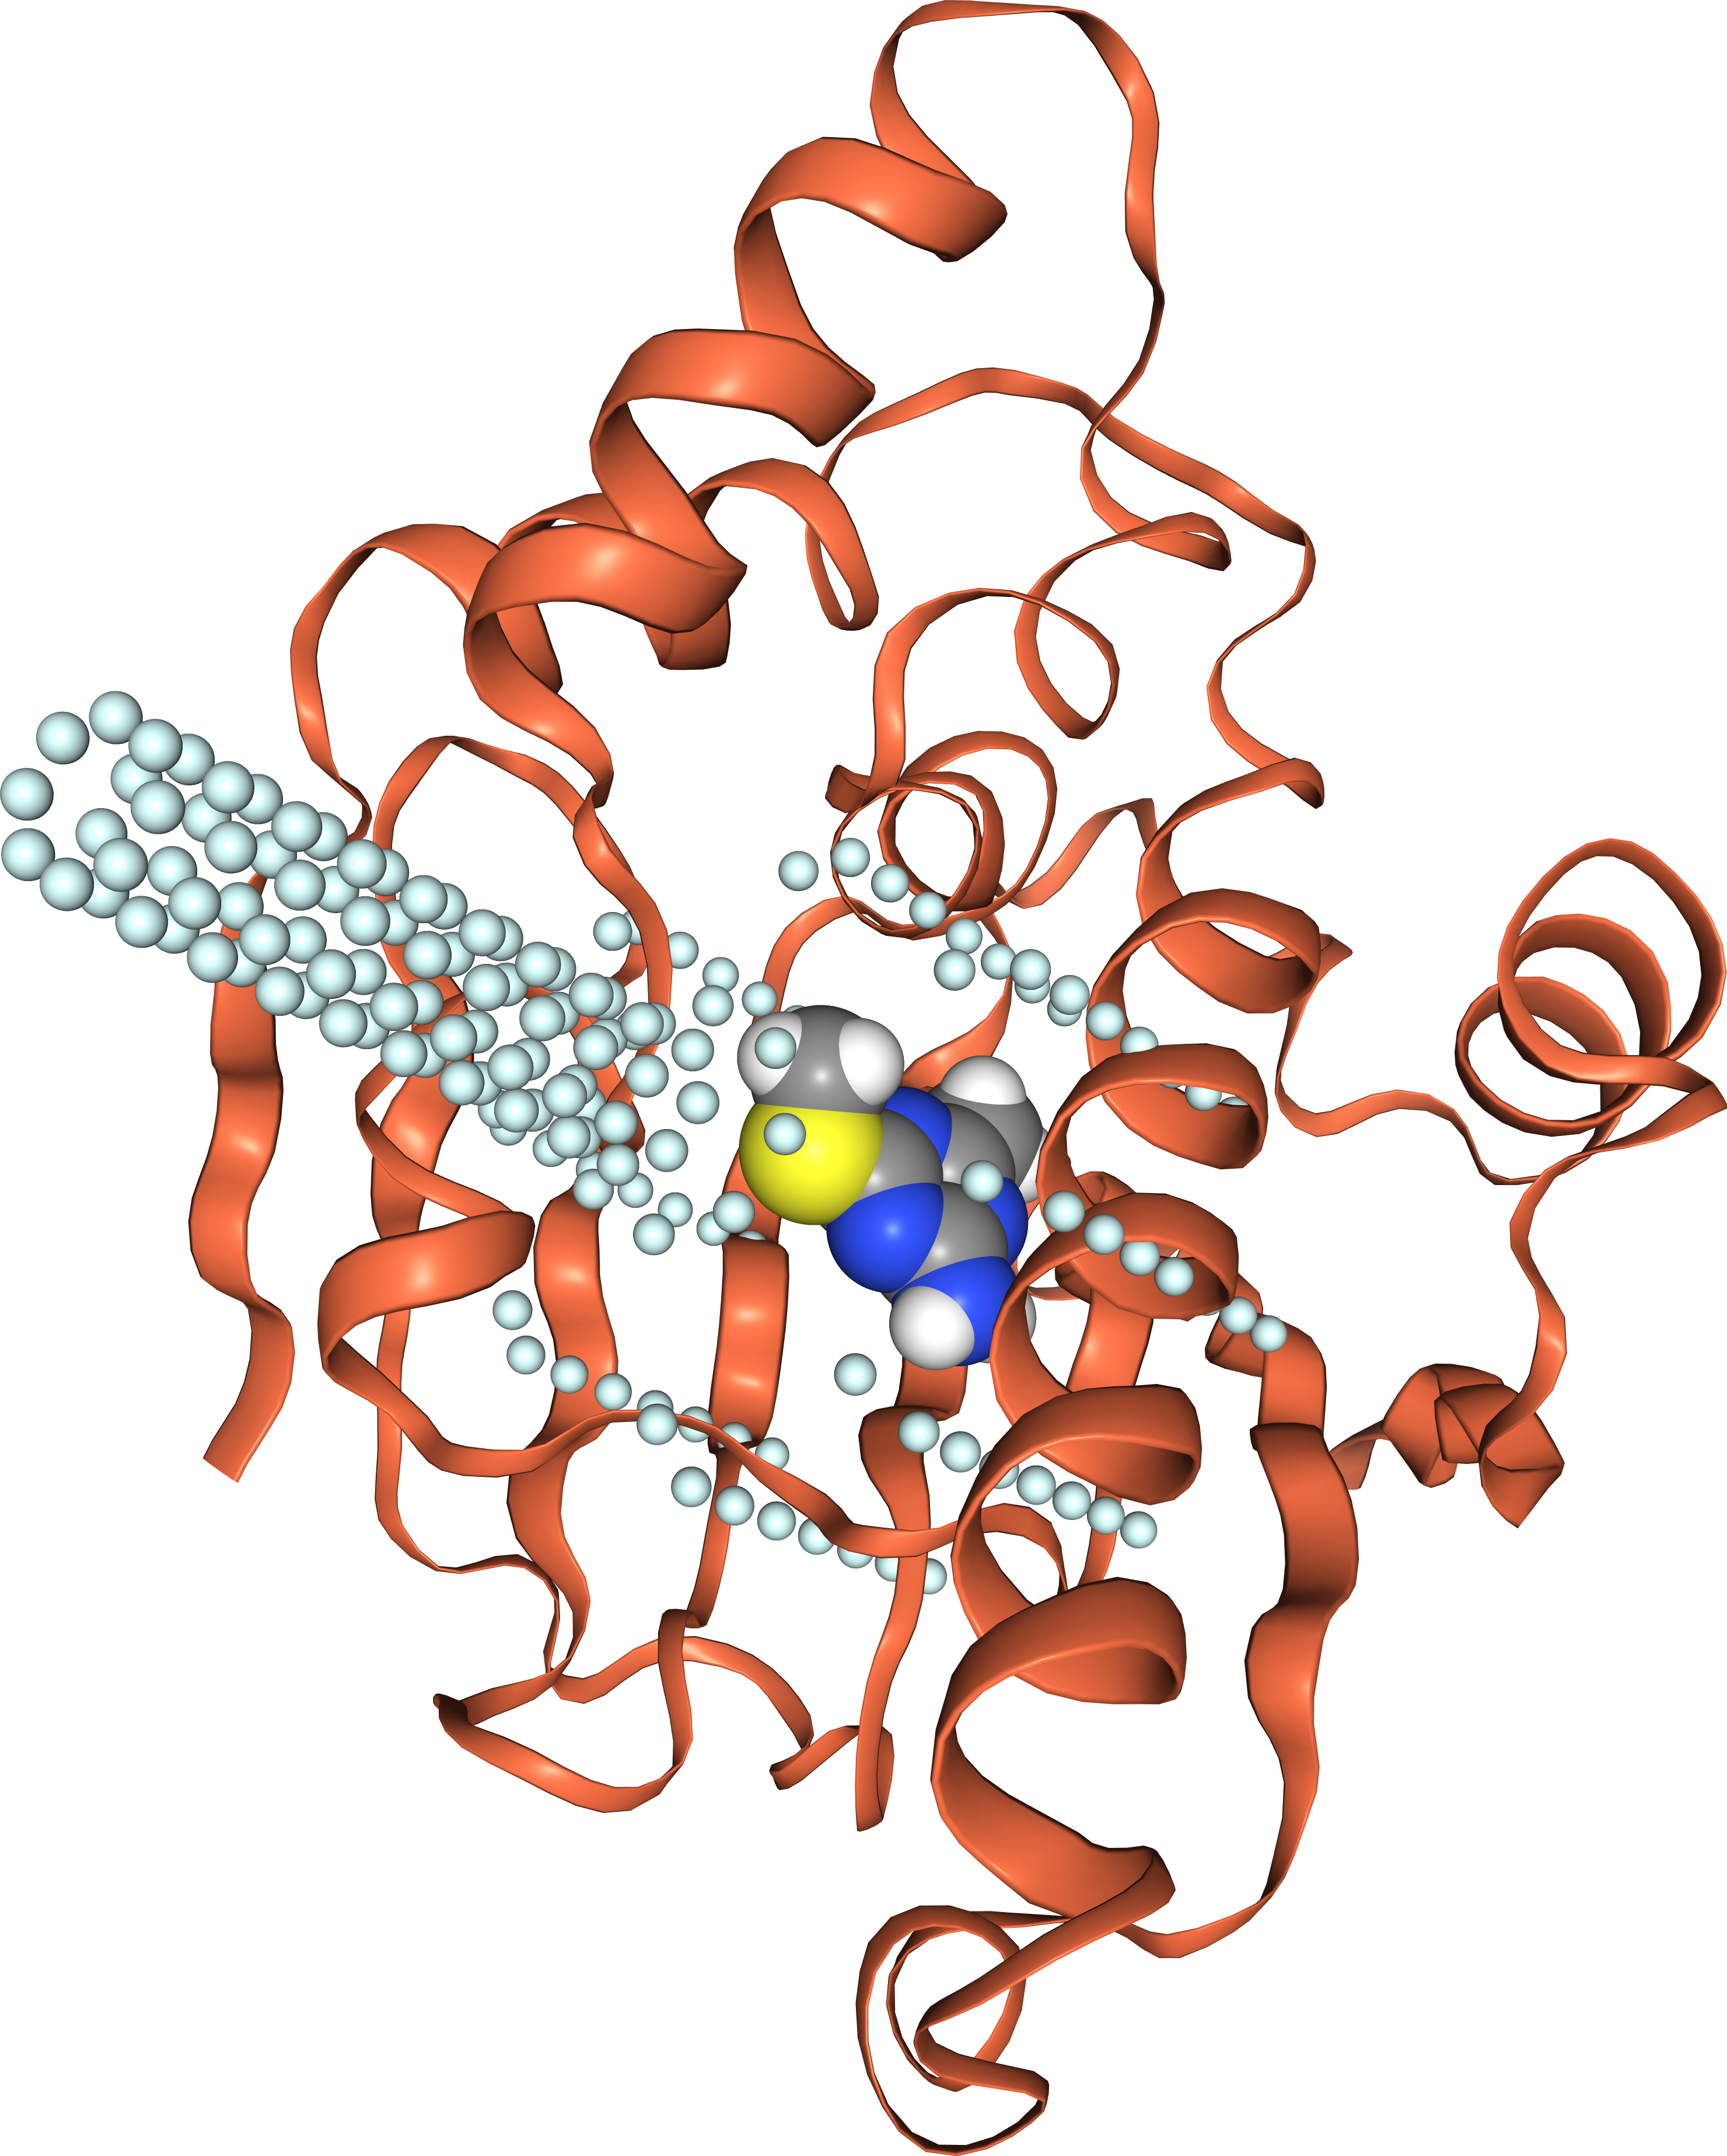
\includegraphics[width=\linewidth]{LIVECOMS/02_funnel_metad/funmetad-hsp90.png}
\caption{Visualisation of funnel restraints autogenerated by BioSimSpace for a HSP90 protein-ligand system.}
\label{fig:fun-hsp90}
\end{figure}

The notebook is demonstrated with a fully solvated HSP90 protein-ligand system originally setup from PDBID:2WI2. 
Figure \ref{fig:fun-hsp90} depicts a rendered funnel overlayed on the HSP90 protein-ligand system in the Jupyter Notebook. The funnel vector is clearly pointing out into the solvent, with no protein residues blocking the way. The default radius is sufficient to encompass the binding site, excluding the rest of the protein.


To obtain converged free energies we recommend simulations of the order of 500 - 2000 ns sampling time. This is best done out of a notebook. For convenience we also \href{https://github.com/OpenBioSim/BioSimSpaceTutorials/tree/main/02_funnel_metad/example_nodes}{provide with this tutorial} as companion resource an LSF submission script that re-implements the notebook functionality in a set of BioSimSpace nodes.  

\hypertarget{analysis}{%
\subsubsection{Analysing funnel metadynamics simulations}\label{analysis}}

The second notebook of this tutorial  \href{https://github.com/OpenBioSim/BioSimSpaceTutorials/blob/main/02_funnel_metad/02_bss-fun-metad-analysis.ipynb}{02-bss-fun-metad-analysis} describes how to analyze a funnel metadynamics simulation. The precision of the ABFE estimate derived from a funnel metadynamics run is linked to the convergence of the free energy profile along the collective variables that define the funnel. The notebook uses provided sample trajectories to show how the range of CV values sampled during a trajectory and two-dimensional free energy surfaces can be plotted with the help of \href{https://biosimspace.openbiosim.org/api/index_Notebook.html}{BSS.Notebook}. The notebook also shows how to compute funnel correction terms using BSS, and how to perform convergence analysis of the absolute binding free energies for different trajectories. Selected visualizations generated by the notebook are depicted in Figure~\ref{fig:fun-hsp90-analyses}. 

\begin{figure}[htp]
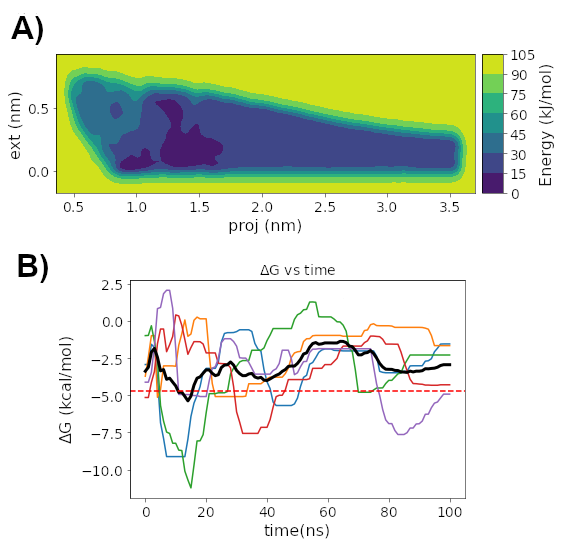
\includegraphics[width=\linewidth]{LIVECOMS/02_funnel_metad/fun-hsp90-analyses.png}
\caption{Selected analyses of funnel metadynamics simulations of the HSP90 protein-ligand system. A) Reconstructed two-dimensional free energy profile from a sample 100 ns trajectory. B) Convergence plots for five replicates of a 100-ns trajectory. The bold black line denotes the mean of the replicates, and the dashed red line the experimental estimate of the absolute binding free energy of the ligand.}
\label{fig:fun-hsp90-analyses}
\end{figure}

